\documentclass[10pt,a4paper]{article}
\author{Harry Armitage}

%\usepackage[utf8]{inputenc}
\usepackage{amsmath}
\usepackage{amsfonts}
\usepackage{amssymb}
\usepackage{amsthm}
\usepackage{float}
\usepackage{mathtools}
\usepackage{geometry}[margin=1in]
\usepackage{xspace}
\usepackage{tikz}
\usepackage{mathrsfs}
\usetikzlibrary{shapes, arrows, decorations.pathmorphing, ducks, automata}
\usepackage[parfill]{parskip}
\usepackage{subcaption}
\usepackage{stmaryrd}
\usepackage{marvosym}
\usepackage{dsfont}
\usepackage{pgfplots}
\usepackage{enumitem}
\usepackage{calc}
\usepackage{tikz-cd}
\usepackage{hyperref}
\usepackage[usestackEOL]{stackengine}

\usepackage{fontspec}
\usepackage{newpxtext, newpxmath}
\usepackage{anyfontsize}

\hypersetup{
    colorlinks,
    citecolor=black,
    filecolor=black,
    linkcolor=black,
    urlcolor=black
}

\newcommand{\f}[1]{\mathfrak{#1}}
\newcommand{\p}{\f{p}}

\newcommand{\st}{\text{ s.t. }}
\newcommand{\contr}{\lightning}
\newcommand{\im}{\mathfrak{i}}
\newcommand{\R}{\mathbb{R}}
\newcommand{\Q}{\mathbb{Q}}
\renewcommand{\C}{\mathbb{C}}
\newcommand{\F}{\mathbb{F}}
\newcommand{\K}{\mathbb{K}}
\newcommand{\N}{\mathbb{N}}
\newcommand{\Z}{\mathbb{Z}}
\renewcommand{\P}{\mathbb{P}}
\renewcommand{\H}{\mathds{H}}
\renewcommand{\O}{\mathcal{O}}
\newcommand{\A}{\mathbb{A}}
\newcommand{\D}{\mathbb{D}}
\renewcommand{\G}{\mathbb{G}}
%\newcommand{\nequiv}{\not\equiv}
\newcommand{\powset}{\mathcal{P}}
\renewcommand{\th}[1][th]{\textsuperscript{#1}\xspace}
\newcommand{\from}{\leftarrow}
\newcommand{\legendre}[2]{\left(\frac{#1}{#2}\right)}
\newcommand{\ow}{\text{otherwise}}
\newcommand{\imp}[2]{\underline{\textit{#1.}$\implies$\textit{#2.}}}
\let\oldexists\exists
\let\oldforall\forall
\renewcommand{\exists}{\oldexists\;}
\renewcommand{\forall}{\;\oldforall}
\renewcommand{\hat}{\widehat}
\renewcommand{\tilde}{\widetilde}
\newcommand{\one}{\mathds{1}}
\newcommand{\under}{\backslash}
\newcommand{\injection}{\hookrightarrow}
\newcommand{\surjection}{\twoheadrightarrow}
\newcommand{\isomarrow}{\mathrel{\setstackgap{S}{-0.5pt}\ensurestackMath{\Shortstack{\scriptstyle\sim\\ \longrightarrow}}}}
\newcommand{\jacobi}{\legendre}
\newcommand{\floor}[1]{\lfloor #1 \rfloor}
\newcommand{\ceil}[1]{\lceil #1 \rceil}
\newcommand{\cbrt}[1]{\sqrt[3]{#1}}
\renewcommand{\angle}[1]{\langle #1 \rangle}
\newcommand{\dbangle}[1]{\angle{\angle{#1}}}
\newcommand{\wrt}{\text{ w.r.t. }}
\newcommand{\abs}[1]{\lvert#1\rvert}
\newcommand{\norm}[1]{\lVert#1\rVert}
\newcommand*\circled[1]{\tikz[baseline=(char.base)]{
      \node[shape=circle,draw,inner sep=2pt] (char) {#1};}
}
\renewcommand{\epsilon}{\varepsilon}
\newcommand{\trianglerightneq}{\mathrel{\ooalign{\raisebox{-0.5ex}{\reflectbox{\rotatebox{90}{$\nshortmid$}}}\cr$\triangleright$\cr}\mkern-3mu}}
\newcommand{\triangleleftneq}{\mathrel{\reflectbox{$\trianglerightneq$}}}

\DeclareMathOperator{\ex}{ex}
\DeclareMathOperator{\id}{id}
\DeclareMathOperator{\upper}{Upper}
\DeclareMathOperator{\dom}{dom}
\DeclareMathOperator{\disc}{disc}
\DeclareMathOperator{\charr}{char}
\DeclareMathOperator{\Image}{im}
\DeclareMathOperator{\ord}{ord}
\DeclareMathOperator{\lcm}{lcm}
\DeclareMathOperator{\aut}{Aut}
\DeclareMathOperator{\diag}{diag}
\DeclareMathOperator{\stab}{stab}
\DeclareMathOperator{\trace}{trace}
\DeclareMathOperator{\ecl}{ecl}
\DeclareMathOperator{\Span}{Span}
\DeclareMathOperator{\Gal}{Gal}
\DeclareMathOperator{\Aut}{Aut}
\DeclareMathOperator{\Frob}{Frob}
\DeclareMathOperator{\Det}{Det}
\let\div\relax
\DeclareMathOperator{\div}{div}
\DeclareMathOperator{\Div}{Div}
\let\Re\relax
\let\Im\relax
\DeclareMathOperator{\Re}{\mathfrak{Re}}
\DeclareMathOperator{\Im}{\mathfrak{Im}}
\DeclareMathOperator{\Frac}{Frac}
\DeclareMathOperator{\Pic}{Pic}
\DeclareMathOperator{\ann}{ann}
\DeclareMathOperator{\Ass}{Ass}
\DeclareMathOperator{\intt}{int}
\DeclareMathOperator{\Hom}{Hom}
\DeclareMathOperator{\End}{End}
\DeclareMathOperator{\tr}{tr}
\DeclareMathOperator{\Tr}{Tr}
\DeclareMathOperator{\Spec}{Spec}
\DeclareMathOperator{\height}{ht}
\DeclareMathOperator{\rank}{rank}
\DeclareMathOperator{\Art}{Art}
\DeclareMathOperator{\gr}{gr}
\DeclareMathOperator{\Tor}{Tor}
\DeclareMathOperator{\Ext}{Ext}
\DeclareMathOperator{\coker}{coker}

\let\emph\relax
\DeclareTextFontCommand{\emph}{\bfseries\em}

\newtheorem{theorem}{Theorem}[section]
\newtheorem{lemma}[theorem]{Lemma}
\newtheorem{corollary}[theorem]{Corollary}
\newtheorem{proposition}[theorem]{Proposition}
\newtheorem{conjecture}[theorem]{Conjecture}
\newtheorem{definition}[theorem]{Definition}

\definecolor{burgundy}{rgb}{0.5, 0.0, 0.13}

\tikzset{sketch/.style={decorate,
 decoration={random steps, amplitude=1pt, segment length=5pt},
 line join=round, draw=black!80, very thick, fill=#1
}}


\title{Modular Forms}
\begin{document}
\maketitle
\tableofcontents
\newpage
\setcounter{section}{-1}
\section{Introduction}
\textbf{Notation.} We will write $\H \coloneqq \{\tau \in \C: \Im(\tau) > 0\}$ for the complex upper half plane. This is acted on by two groups: \[GL_2(\R)^+ = \{g \in GL_2(\R): \det(g) > 0\} \geq SL_2(\Z) = \{g \in GL_2(\Z) : \det(g)=1\}\]
\begin{lemma}
  $GL_2(\R)^+$ acts on $\H$ by M\"obius transformations. This action is transitive.
\end{lemma}
\begin{proof}
  Let $\tau \in \H, g = \begin{pmatrix} a&b\\c&d\end{pmatrix} \in GL_2(\R)^+$. We then write $g\tau = \frac{a\tau+b}{c\tau+d}$. This is an action on $\C$ by theory about M\"obius transformations. To see that $g\tau \in \H$, we check:
  \[\Im(g\tau) = \frac{1}{2}(g\tau - \overline{g\tau}) = \det(g) \frac{\Im(\tau)}{|c\tau+d|^2}\]

  Now for transitivity, let $\tau = x+\im y \in \H$. Then $\tau = \begin{pmatrix}y&x\\0&1\end{pmatrix}\im$.
\end{proof}
\begin{definition}
  Let $k \in \Z$, and $f : \H \to \C\cup\{\infty\}$, and let $g \in GL_2(\R)^+$. Then we define $f|_k[g]:\H \to \C\cup\{\infty\}$ by the formula
  \[f|_k[g](\tau) = f(g\tau)\det(g)^{k-1}j(g, \tau)^{-k}\]
  where $j(g, \tau) = c\tau+d$.
\end{definition}
\begin{lemma}
  This defines a right actions of $GL_2(\R)^+$ on the set of functions $f:\H \to \C\cup\{\infty\}$.
\end{lemma}
\begin{proof}
  Suppose $g, h \in GL_2(\R)^+$. We need to show that $f|_k[gh] = (f|_k[g])|_k[h]$.
  \begin{align*}
    RHS(\tau) &= f|_k[g](h\tau)\det(h)^{k-1}j(h, \tau)^{-k}\\
    &= f(gh\tau)\det(g)^{k-1}j(g, h\tau)^{-k}j(h,\tau)^{-k}\det(h)^{k-1}\\
    LHS(\tau) &= f(gh\tau)\det(gh)^{k-1}j(gh,\tau)
  \end{align*}
  So we need to check that $j(g, h\tau)j(h,\tau) = j(gh,\tau)$.

  Note that if $g = \begin{pmatrix}a&b\\c&d\end{pmatrix}$, then $g\begin{pmatrix}\tau\\1\end{pmatrix} = \begin{pmatrix}a\tau+b\\c\tau+d\end{pmatrix} = j(g,\tau)\begin{pmatrix}g\tau\\1\end{pmatrix}$.

  So $gh\begin{pmatrix}\tau\\1\end{pmatrix} = j(gh,\tau)\begin{pmatrix}gh\tau\\1\end{pmatrix} = gj(h,\tau)\begin{pmatrix}h\tau\\1\end{pmatrix} = j(h,\tau)j(g,h\tau)\begin{pmatrix}gh\tau\\1\end{pmatrix}$.
\end{proof}
\begin{definition}
  Let $k \in \Z$, and let $\Gamma \leq SL_2(\Z)$ be a finite index subgroup. Then a meromorphic function $f:\H \to \C \cup\{\infty\}$ is called a weakly modular function of weight $k$ and level $\Gamma$ if it satisfies $\forall \gamma \in \Gamma, f|_k [\gamma] = f$.
\end{definition}

\textbf{Motivating Examples}
\begin{enumerate}
  \item Modular forms were first studied in the context of elliptic functions. Suppose that $E$ is an elliptic curve over $\C$, and let $\omega$ be a non-vanishing holomorphic differential on $E$. Then there's a unique holomorphic isomorphism of Riemann surfaces
  \[\C/\Lambda \xrightarrow[\psi]{\sim} E(\C)\]
  such that $\psi^{\ast}(\omega) = dz$. Here $\Lambda\subset\C$ is a lattice.

  $E$ can be defined by the equation $y^2=x^3-60G_4(\Lambda)x-140G_6(\Lambda)$ where $G_k(\Lambda) = \sum\limits_{\omega \in \Lambda\setminus\{0\}}\omega^{-k}$. This is absolutely convergent provided $k \geq 4$.

  If $\tau \in \H$, then we can write $\Lambda_\tau = \Z\tau \oplus \Z$. This is a lattice, and the functions $G_k(\tau) = G_k(\Lambda \tau)$ are examples of modular forms.

  \item If $f:\H \to \C$ is a modular form, then $f$ has a Fourier expansion $f(\tau) = \sum\limits_{n\geq 0}a_n e^{2\pi\im n\tau/h}$ for some natural number $h$, and complex numbers $a_n$. These Fourier coefficients often carry useful arithmetic information.

  For example, consider $\theta(\tau) = \sum\limits_{n \in \Z}e^{\pi\im n^2\tau}$. If $k \geq 2$ is an even integer, then $\theta^{2k}$ is a modular form of weight $k$. Its Fourier expansion is $\theta^{2k}(\tau) = \sum\limits_{n \geq1}r_{2k}(n)e^{\pi\im n \tau}$ where $r_{2k}(n)$ is the number of ways of writing $n = x_1^2 + \ldots x_{2k}^2$, where $x_i \in \Z$.

  By relating $\theta^{2k}$ to other modular forms with known Fourier series, we can then get information about the numbers $r_{2k}(n)$. For example, $r_4(n) = 8\sum\limits_{d|n, 4\nmid d} d$.

  \item Recall the Riemann zeta function $\zeta(s) = \sum_{n\geq 1}n^{-s}$. This function has some important properties:
  \begin{enumerate}[label=\alph*)]
    \item It has a meromorphic continuation to all of $\C$.
    \item It has a functional equation relating $\zeta(s)$ and $\zeta(1-s)$.
    \item It has a representation as an Euler product $\zeta(s) = \prod_{p}(1-p^{-s})^{-1}$.
  \end{enumerate}
  Any series $L(s) = \sum_{n\geq 1}a_n n^{-s}$ with $a_n \in \C$ which has properties analogous to these is called an $L$-function.

  For example, if $N \in \N$ and $\chi: (\Z/N\Z)^\times \to \C^\times$ is a character, we can define the Dirichlet $L$-function $L(\chi, s) = \sum_{(n,N)=1} \chi(n \mod N)n^{-s}$. These functions can be used to prove Dirichlet's theorem on primes in arithmetic progression.

  Modular forms can be used to construct $L$-functions with these properties. To find the right modular forms, we need to introduce Hecke operators.

  \item The Langlands programme predicts relations between objects ocurring in number theory and modular forms. This includes as a special case the Shimura-Taniyama-Weil conjecture, otherwise known as the modularity theorem. This asserts a bijection between elliptic curves over $\Q$ up to isogeny and certain modular forms, given by ($L$-function of elliptic curve) = ($L$-function of modular form).
\end{enumerate}
\section{Modular forms on $SL_2(\Z)$}
Recall the definition, for $f:\H \to \C, k \in \Z, g \in GL_2(\R)^+$, we have
\[f|_k[g](\tau) = \det(g)^{k-1}f(g\tau)j(g,\tau)^{-k}\]
We said $f$ is \emph{weakly modular of weight k and level $SL_2(\Z)$} if $f$ is meromorphic on $\H$ and, for all $\gamma \in SL_2(\Z)$, $f|_k[\gamma] = f$.

Note that $T = \begin{pmatrix}1&1\\0&1 \end{pmatrix} \in SL_2(\Z)$ satisfies $f|_k[T](\tau) = f(\tau+1)$. So if $f$ is a weakly modular function, then we can define a new function
\[\tilde{f}:\{q \in \C: 0<|q|<1\} \to \C; e^{2\pi\im\tau} \mapsto f(\tau)\]
This function $\tilde{f}$ is meromorphic, since $f$ is.
\begin{definition}
  We say that the weakly modular function $f$ is:
  \begin{itemize}
    \item meromorphic at $\infty$ if $\tilde{f}$ is meromorphic at 0.
    \item holomorphic at $\infty$ if $\tilde{f}$ is holomorphic at 0.
    \item vanishes at $\infty$ if $\tilde{f}$ is holomorphic and vanishes at 0.
  \end{itemize}
\end{definition}
If $f$ is meromorphic at $\infty$ then $\tilde{f}$ has a Laurent expansion $\tilde{f}(q) = \sum_{n \in \Z}a_nq^n$ valid in some region $\{0 <|q|< \epsilon\}$, where $a_n \in \C$ and $a_n = 0$ if $n<0$ and $|n|$ is sufficiently large.

We get a formula $f(\tau) = \sum_{n\in \Z}a_nq^n$ where $q = e^{2\pi\im\tau}$. This is valid in some region $\{\tau \in \H : \Im \tau > R\}$, and is called the $q$-expansion of $f$. Then $f$ is holomorphic at $\infty$ if and only if $a_n = 0$ when $n < 0$, and $f(\infty) = a_0$.
\begin{definition}
  Let $f$ be a weakly modular function of weight $k$ and level $SL_2(\Z)$. We say that $f$ is
  \begin{itemize}
    \item a \emph{modular function} if $f$ is meromorphic at $\infty$.
    \item a \emph{modular form} if $f$ is holomorphic in $\H$ and holomorphic at $\infty$.
    \item a \emph{cuspidal modular form} if $f$ is a modular form vanishing at $\infty$.
  \end{itemize}
  all with weight $k$ and level $SL_2(\Z)$.

  We write $M_k(SL_2(\Z))$ for the $\C$-vector space of modular forms of weight $k$ and level $SL_2(\Z)$. We write $S_k(SL_2(\Z))$ for the subspace of cuspidal modular forms.
\end{definition}
\textbf{Examples.} If $\tau \in \H$, then $\Lambda_\tau = \Z\tau \oplus \Z$. if $k \in \Z$, then we can define $G_k(\tau) = \sum\limits_{\omega \in \Lambda_\tau\setminus\{0\}}\omega^{-k}$.

If $\gamma = \begin{pmatrix}a&b\\c&d\end{pmatrix} \in SL_2(\Z)$, then $\Lambda_{\gamma \tau} = \Z\left(\frac{a\tau+b}{c\tau+d}\right)\oplus \Z = j(\gamma,\tau)^{-1}\Z(a\tau+b)\oplus \Z(c\tau+d) = j(\gamma,\tau)^{-1}\Lambda_\tau$.

Finally, we find $G_k|_k[\gamma](\tau) = G_k(\gamma\tau)j(\gamma,\tau)^{-k} = \sum\limits_{\omega \in \Lambda_{\gamma\tau}\setminus\{0\}}(\omega j(\gamma,\tau))^{-k} = \sum\limits_{\omega \in \Lambda_\tau\setminus\{0\}} \omega^{-k} = G_k(\tau)$.
\begin{proposition}
  Suppose $k \geq 4$ and $k$ is even. Then $G_k(\tau)$ converges absolutely and uniformly on compact subsets of $\H$. Moreover, $G_k(\tau)$ is holomorphic at $\infty$ and $G_k(\infty) = 2\zeta(k)$. In particular, $G_k \in M_k(SL_2(\Z))$.
\end{proposition}
\textbf{Remark.} We have $-I = \begin{pmatrix} -1&0\\0&-1 \end{pmatrix} \in SL_2(\Z)$ and $f|_k[-I] = f\cdot(-1)^k$, so if $k$ were odd then $f \equiv 0$, and hence $M_k(SL_2(\Z)) = 0$ when $k$ is odd.
\begin{proof}
  Fix $A \geq 1$. Define $\Omega_A = \{\tau \in \H : |\Re(|\tau)|\leq A, \Im(\tau) \geq \frac{1}{A}\}$. We'll show uniform convergence of $G_k$ in $\Omega_A$. Note that if $\tau \in \Omega_A$, then for any $x \in \R$, $|\tau+x| \geq \frac{1}{A}$, and $|\tau+x| \geq \frac{1}{2}|x|$ if $|x|\geq 2A$. Hence $|\tau+x| \geq \sup(1/A, 1/2A^2|x|) \geq \frac{1}{2A^2}\sup(1, |x|)$ for any $x \in \R$.

  If $\tau \in \Omega_A$, then:
  \begin{align*}
    \sum_{(m,n) \in \Z^2\setminus\{0\}} |m\tau+n|^{-k} &= \sum_{(m,n)} |m|^{-k}|\tau+n/m|^{-k} \\
    &\leq \sum_{(m,n)}\frac{|m|^{-k}}{(2A)^{-k}}\sum(1, |n/m|)^{-k}\\
    &= \sum_{(m,n)}(2A)^k \sup(|m|^{-k}, |n|^{-k})\\
    &= \sum_{r \in \N} (2A)^k r^k 8r = (2A)^k8\zeta(k-1)
  \end{align*}
  This shows absolute and uniform convergence.

  To show that $G_k$ is holomorphic at $\infty$ and $G_k(\infty) = 2\zeta(k)$, it's enough to show that
  \[\lim_{\tau\in\Omega_1, \Im\tau\to\infty} G_k(\tau) = 2\zeta(k)\]
  This limit equals $\sum\limits_{(m,n)}\lim\limits_{\Im\tau\to\infty}(m\tau+n)^{-k} = \sum\limits_{n\in \Z\setminus \{0\}}n^{-k} = 2\zeta(k)$, as all terms with $m \neq 0$ vanish.
\end{proof}
$G_k$ is an example of an \emph{Eisenstein series}.
\begin{definition}
  We define the \emph{normalised Eisenstein series} $E_k(\tau) = \frac{1}{2\zeta(k)}G_k(\tau) = 1 + \sum_{n\geq 1}a_nq^n$. We'll see that the $a_n$ are rational numbers of bounded denominators.
\end{definition}
\textbf{Remark.} If $f \in M_k(SL_2(\Z))$ and $g \in M_\ell(SL_2(\Z))$, then $fg \in M_{k+\ell}(SL_2(\Z))$. So $E_4^3, E_6^2 \in M_{12}(SL_2(\Z))$, and $E_4^3(\infty) = E_6^2(\infty)$, so $\Delta = \frac{E_4^3-E_6^2}{1728} \in S_{12}(SL_2(\Z))$. We'll see shortly that $\Delta = \sum_{n\geq 1} b_nq^n$ where $b_1 = 1, b_n \in \Z$ for all $n \geq 1$.

We now study a fundamental domain for the action of $SL_2(\Z)$ on $\H$. We will write $\Gamma(1) = SL_2(\Z)$, and $\overline{\Gamma(1)} = SL_2(\Z)/\angle{-I}$. This will make sense later.

We write \[\mathscr{F} = \{\tau \in \H : -\frac12 \leq \Re\tau \leq \frac12, |\tau|\geq 1\}\] and \[\mathscr{F}' = \{\tau \in \mathscr{F} : \Re \tau < 1/2, |\tau| = 1 \implies \Re\tau \leq 0\}\]
In the following diagram, $\mathscr{F}$ is all of the green + orange regions, whilst $\mathscr{F}'$ is just the green area. We also define $\rho\coloneqq \exp(2\pi\im/3)$
\begin{center}
  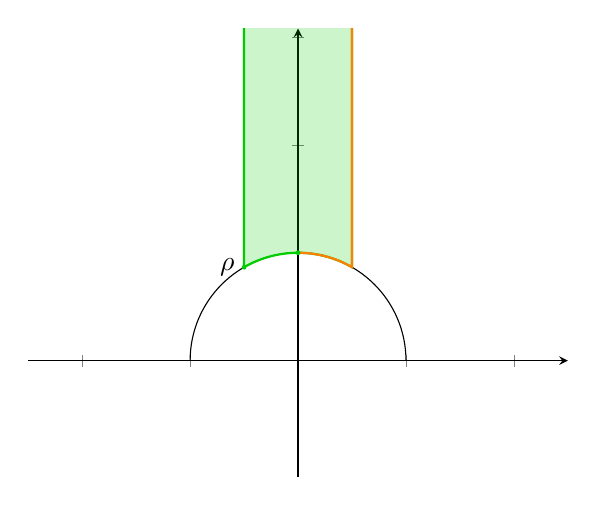
\begin{tikzpicture}
    \begin{axis}[
      xmin=-2.5, xmax=2.5,
      ymin=-0.5, ymax=2.5,
      axis lines=middle,
      axis equal,
      xtick={-4,-3,...,4},
      xticklabels = \empty,
      ytick={0,1,...,4},
      yticklabels = \empty,
      ]
      \draw (-1,0) arc (180:0:1);
      \draw[thick, green!80!black, fill=green!80!black, fill opacity=0.2] (-0.5,4.5) -- (-0.5,0.866) arc (120:60:1) -- (0.5,4.5) -- cycle;
      \draw[thick, orange] (0,1) arc (90:60:1) -- (0.5,4.5);
      \fill[green!80!black] (0,1) circle (0.3mm);
      \fill[green!80!black] (-0.5,0.866) circle (0.3mm);
      \node[left] at (-0.5,0.866) {$\rho$};
    \end{axis}
  \end{tikzpicture}
\end{center}
We have elements $T = \begin{pmatrix} 1&1\\0&1\end{pmatrix}$ and $S =\begin{pmatrix}0&-1\\1&0\end{pmatrix}\in \Gamma(1)$.
\begin{proposition}
  $\mathscr{F}$ is a fundamental domain for the action of $\overline{\Gamma(1)}$ on $\H$. More precisely, if $\tau\in\H$ there is $\gamma \in \overline{\Gamma(1)}$ such that $\gamma\tau \in \mathscr{F}$. If $\gamma \tau \in \mathscr{F}^\circ$, then $\gamma$ is unique. Moreover, each $\tau \in \H$ is $\overline{\Gamma(1)}$-conjugate to exactly one element of $\mathscr{F}'$.
\end{proposition}
\begin{proof}
  We first prove that any $\tau \in \H$ is $\overline{\Gamma(1)}$-conjugate to an element of $\mathscr{F}$. We proved earlier that if $\tau \in \H$ and $\gamma \in \Gamma(1)$, then $\Im \gamma(\tau) = \Im(\tau)/|c\tau+d|^2$.

  If $\tau \in \H$, then $\Lambda_\tau = \Z_\tau \oplus \Z$ is a lattice. So as $(c,d) \in \Z^2\setminus\{0\}$, the numbers $|c\tau+d|$ achieve a minimum. Consequently, the numbers $\Im \gamma(\tau)$ for $\gamma \in \Gamma(1)$ achieve a maximum. So \textsc{wlog} we may assume $\Im(\tau) \geq \Im(\gamma \tau)$ for all $\gamma \in \Gamma(1)$. Also \textsc{wlog} we may take $-\frac12 \leq \Re(\tau) \leq \frac12$.

  We then claim that these properties are sufficient for $\tau \in \mathscr{F}$. It is sufficient to show that $|\tau| \geq 1$. We have $\Im(S\tau) = \Im(\tau)/|\tau|^2 \leq \Im(\tau)$, and hence $|\tau|^2 \geq 1$, so we are done.
\end{proof}
We slightly strengthen this with the following proposition:
\begin{proposition}\hspace*{0cm}
  \begin{enumerate}
    \item For all $\tau \in \H$, there is a unique $\gamma \in \overline{\Gamma(1)}$ such that $\gamma \tau \in \mathscr{F}'.$
    \item If $\tau \in \mathscr{F}'$, then $\Stab_{\overline{\Gamma(1)}}(\tau) = \{I\}$, except $\Stab_{\overline{\Gamma(1)}}(\im) = \{I, S\}$ and $\Stab_{\overline{\Gamma(1)}}(\rho) = \{1,ST,(ST)^2\}$.
    \item $\overline{\Gamma(1)}$ is generated by $S$ and $T$.
  \end{enumerate}
\end{proposition}
\begin{proof}
  To prove the first two parts, it's enough to show that:
  \begin{enumerate}[label=\alph*)]
    \item For all $\tau \in \H$, there is $\gamma \in \overline{\Gamma(1)}$ such that $\gamma\tau \in \mathscr{F}'$.
    \item For all $\tau, \tau' \in \mathscr{F}'$ and $\gamma \in \overline{\Gamma(1)}$, $\gamma\tau'=\tau \implies \tau'=\tau$ and either $\begin{cases} \gamma=1\\\tau=\im, \gamma=S\\\tau=\rho, \gamma=ST, (ST)^2\end{cases}$.
  \end{enumerate}
  a) was done above. For b), take $\tau,\tau' \in \mathscr{F}'$ such that $\tau' = \gamma\tau$. We have $\Im(\gamma\tau) = \Im(\tau)/|c\tau+d|^2$ where $\gamma = \begin{pmatrix}a&b\\c&d\end{pmatrix}$.

  Without loss of generality, we have $\Im(\tau') = \Im(\gamma\tau) \geq \Im(\tau)\implies |c\tau+d|\leq 1$.

  So $\Im(\tau) \geq \sqrt{3}/2 \implies |c\tau+d| \geq c\sqrt{3}/2$, and so $|c| \leq 1$, so we can assume $c = 1$ or $0$ (if $-1$, just multiply by $-I$, since we are in $\overline{\Gamma(1)} = \Gamma(1)/\angle{-I}$). We then split into cases:
  \begin{enumerate}
    \item $c = 0, \gamma = \begin{pmatrix}1&b\\0&1\end{pmatrix}$. This forces $\gamma = I, \tau=\tau'$.
    \item $c = 1, \gamma = \begin{pmatrix}a&b\\1&d\end{pmatrix}$. Now $|\tau+d| \leq 1$. Then $\tau \in \mathscr{F}' \implies$ either $d = 0, |\tau| = 1$, or $d = 1, \tau=\rho$.

    In the first case, $\gamma = \begin{pmatrix} a&-1\\1&0\end{pmatrix}$, and so $\gamma\tau = a-\frac1\tau$. We have $\Re(\tau), \Re(\Gamma(\tau)) = a - \Re(\tau)$ both in $[-1/2,0]$. The only possibilities are $\Re(\tau) = -\frac12, a = -1, \tau=\rho, \gamma=(ST)^2$ and $\Re(\tau) = 0, a = 0, \tau = \im, \gamma=S$.

    In the second case, $d = 1, \tau  = \rho, \gamma=\begin{pmatrix}a&b\\1&1\end{pmatrix}$. Then $\gamma\rho = \frac{a\rho+b}{\rho + 1}$. We have $\rho^2+\rho+1 = 0, \rho^2 = \rho{-1}$, so $\gamma\rho = -\rho(a\rho+b) = -a\rho^{-1}-b\rho$.

    We know that $|\rho + 1| = |\tau+d| = 1$, so $\Im(\gamma\rho) = \Im(\rho)/|\rho+1| = \Im(\rho)$. So $\gamma\rho = \rho$, as $\rho$ is the unique element of $\mathscr{F}'$ of smallest imaginary part, and hence $\rho = -a\rho^{-1}-b\rho\implies a=0, b = -1$, and so $\gamma = ST$.
  \end{enumerate}

  For part 3., lets take $G = \angle{S,T}$. For all $\tau \in \H$, there is $\gamma \in G$ with $\gamma \tau \in \mathscr{F}$. Why? Without loss of generality, we can assume that, for all $\gamma \in G, \Im(\gamma\tau) \leq \Im(\tau)$, and moreover that $-\frac12 \leq \Re(\tau)\leq \frac12$.

  This implies that $\tau \in \mathscr{F}$, as $\Im(S\tau) = \Im(\tau)/|\tau|^2 \leq \Im(\tau) \implies |\tau| \geq 1$.

  Choose $\tau \in \mathscr{F}^\circ$. Choose $\gamma \in \overline{\Gamma(1)}$. We'll show that $\gamma \in G$. Note that $\gamma\tau \in \H$, so there is $\delta \in G$ such that $\delta\gamma\tau \in \mathscr{F}$, so $\delta\gamma\tau \in \mathscr{F}^\circ$ and $\delta\gamma = I$, so $\delta =\gamma^{-1} \in G$.
\end{proof}
If $P \in \overline{\Gamma(1)} \diagdown \H$ (since $\overline{\Gamma(1)}$ acts on the left on $\H$, this is a left quotient. $P$ is a $\overline{\Gamma(1)}$-orbit, i.e. can be represented as $\overline{\Gamma(1)}\cdot \tau$ for some $\tau \in \H$), then we define $e_P = |\Stab_{\overline{\Gamma(1)}}(\tau)|$.

We've just shown that $e_P = 1$ except for $\begin{cases} e_{\overline{\Gamma(1)}\cdot \rho} = e_\rho = 3\\ e_{\overline{\Gamma(1)}\cdot \im} = e_\im = 2\end{cases}$.

Suppose that $f$ is a modular function of weight $k$ and level $SL_2(\Z)$. Then we define $v_P(f)$ to be the order of $f$ at $\tau$ (where $\tau$ is a representative for $P$).

Note that this independent of the specific choice of representative $\tau$ as, for any $\gamma \in \Gamma(1)$ we have $f(\gamma\tau)j(\gamma,\tau)^{-k} = f(\tau)$, and $j(\gamma,\tau)$ is holomorphic and non-vanishing.

We define $v_\infty(f) = \inf \{n\in\Z : a_n \neq 0\}$, where $f(\tau) = \sum_{n\in \Z} a_nq^n$ is the $q$-expansion of $f$. Equivalently, this is the order of $\tilde{f}$ at $q=0$.
\begin{theorem}
  Let $f$ be a modular function of weight $k$ and level $SL_2(\Z)$. Assume that $f\neq 0$. Then:
  \[v_\infty(f) + \sum_{P \in \overline{\Gamma(1)}\diagdown \H} \frac{1}{e_P}v_P(f) = \frac{k}{12}\]
\end{theorem}
\begin{proof}
  Let $U \subseteq \C$ be an open subset, and $\gamma \subseteq U$ a positively oriented simple closed contour, and $f:U \to \C$ a meromorphic function with no zeros or poles on $\gamma$. Then $\frac{1}{2\pi\im}\oint_\gamma\frac{df}{f} = \sum_{\tau \in \Int(\gamma)} v_\tau(f)$ - this is the argument principle.

  Let's first prove the theorem assuming that $f$ has no zeros or poles on the boundary of $\mathscr{F}$. Since $f$ is meromorphic at infinity, there exists a $R > 0$ such that $f$ has no zeros or poles on in $\{\tau \in \H:\Im(\tau) \geq R\}$.

  We consider the contour $\gamma = ABCDEA$:
  \begin{center}
    \begin{tikzpicture}
      \begin{axis}[
        xmin=-1.5, xmax=1.5,
        ymin=-0.5, ymax=2.5,
        xtick={-0.5,0,0.5},
        ytick=\empty,
        xticklabels={$-\frac12$,0,$\frac12$},
        %yticklabels=\empty,
        axis lines=middle,
        axis equal,
      ]
      \begin{scope}[
        thick,
        decoration={markings, mark=at position 0.5 with {\arrow{>}}}
      ]
        \draw[postaction={decorate}] (-0.5,2) -- (-0.5,0.866);
        \draw[postaction={decorate}] (-0.5,0.866) arc(120:60:1);
        \draw[postaction={decorate}] (0.5,0.866) -- (0.5,2);
        \draw[postaction={decorate}] (0.5,2) -- (-0.5,2);
      \end{scope}
      \node[left] at (-0.5,2) {$A$};
      \node[left] at (-0.5,0.866) {$B$};
      \node[above left] at (0,1) {$C$};
      \node[right] at (0.5,0.866) {$D$};
      \node[right] at (0.5,2) {$E$};
      \end{axis}
    \end{tikzpicture}
  \end{center}
  where $A = -\frac12 + \im R, B = \rho, C = \im, D = \rho + 1, E = \frac12 + \im R$.

  The argument principle gives $\frac{1}{2\pi\im}\oint_\gamma \frac{df}{f} = \sum_{\tau \in \Int(\mathscr{F})} v_\tau(f)$.

  We can break up the integral into the different segments AB, BC, CD, DE, and EA, and make some observations:
  \begin{itemize}
    \item $f(\tau) = f(\tau+1)$, so $\int_A^B \frac{df}{f} = \int_E^D \frac{df}{f} = -\int_D^E \frac{df}{f}$, so these paths cancel.
    \item The image of the path $EA$ under the map $\tau \mapsto e^{2\pi\im\tau}$ is a negatively oriented circle $c$ going around $q= 0$, so $\frac{1}{2\pi\im}\int_E^A \frac{df}{f} = \frac{1}{2\pi\im}\oint_c \frac{d\tilde{f}}{\tilde{f}} = -v_0(\tilde{f}) = -v_\infty(f)$.
    \item The path from $CD$ is the image of the path $CB$ under $S$. So $\frac{1}{2\pi\im}\int_D^C \frac{df}{f} = \frac{1}{2\pi\im}\int_B^C \frac{d(f\circ S)}{(f\circ S)}$. We have $f(S\tau) = f(\tau)\tau^k$, so $\frac{d(f\circ S)}{f\circ S} = \frac{kd\tau}{\tau} + \frac{df}{f}$.

    Hence this integral is $\frac{1}{2\pi\im}\int_B^C \frac{k}{\tau}d\tau + \int_B^C \frac{df}{f}$, and so we have:
    \[\frac{1}{2\pi\im}\int_B^C \frac{df}{f} + \frac{1}{2\pi\im}\int_C^D \frac{df}{f} = \frac{1}{2\pi\im}\int_C^B\frac{k}{\tau}d\tau = \frac{k}{12}\]
  \end{itemize}
  Putting this all together, we have:
  \[\frac{k}{12} - v_\infty(f) = \sum_{\tau \in \Int(\mathscr{F})} v_\tau(f)\]
  Since we're assuming all zeros and poles are in the interior and so have $e_P = 1$, adding in the $e_P$s for the result in the theorem doesn't change anything.

  If there are zeros or poles on the boundary of $\mathscr{F}$, then we need a modified contour. First suppose that $f$ has a zero or pole on the lines $AB$ and $DE$, but nowhere else. Then we use the contour $\gamma'$:
  \begin{center}
    \begin{tikzpicture}
      \begin{axis}[
        xmin=-1.5, xmax=1.5,
        ymin=-0.5, ymax=2.5,
        xtick={-0.5,0,0.5},
        ytick=\empty,
        xticklabels={$-\frac12$,0,$\frac12$},
        %yticklabels=\empty,
        axis lines=middle,
        axis equal,
      ]
      \node[left] (A) at (-0.5,2) {$A$};
      \node[left] (B) at (-0.5,0.866) {$B$};
      \node[above left] (C) at (0,1) {$C$};
      \node[right] (D) at (0.5,0.866) {$D$};
      \node[right] (E) at (0.5,2) {$E$};
      \node[burgundy, circle, draw, fill, minimum size=.5pt, inner sep=1pt] (P1) at (-0.5,1.5) {};
      \node[burgundy, circle, draw, fill, minimum size=.5pt, inner sep=1pt] (P2) at (0.5,1.5) {};
      \begin{scope}[
        thick,
        decoration={markings, mark=at position 0.5 with {\arrow{>}}}
      ]
        \draw[postaction={decorate}] (-0.5,2) -- (-0.5,1.55);
        \draw (-0.5,1.55) arc(90:270:0.05);
        \draw[postaction={decorate}] (-0.5,1.45) -- (-0.5,0.866);
        \draw[postaction={decorate}] (-0.5,0.866) arc(120:60:1);
        \draw[postaction={decorate}] (0.5,0.866) -- (0.5,1.45);
        \draw (0.5,1.55) arc(90:270:0.05);
        \draw[postaction={decorate}] (0.5,1.55) -- (0.5,2);
        \draw[postaction={decorate}] (0.5,2) -- (-0.5,2);
      \end{scope}
      \end{axis}
    \end{tikzpicture}
  \end{center}
  where the small semicircles are chosen so that they avoid all zeros or poles of $f$, noting that the zeros and poles of a meromorphic function are isolated, and so that $AB$ is mapped to $ED$ by $T$, in order to still have $\int_B^A \frac{df}{f} + \int_D^E \frac{df}{f} = 0$. The rest of the proof goes through as before. We can make a similar modification if $f$ has a zero/pole on $BC$.

  The remaining case is when $f$ has a zero or pole at $\rho$ or $\im$. In this case, we use the following observation: let $g: U \to \C$ be a meromorphic function defined in an open neighbourhood of $z=0$.

  We consider the paths $\gamma_\epsilon:[0,1] \to U$ given by $\gamma_\epsilon(t) = \epsilon e^{2\pi\im(\theta_0 + t\theta)}$. Then:
  \[\lim_{\epsilon \to 0} \frac{1}{2\pi\im} \int_{\gamma_\epsilon} \frac{dg}{g} = \frac{\theta}{2\pi}v_0(g)\]
  To show this, write $g(z) = z^nh(z)$ where $n = v_0(g)$ and $h(z)$ is holomorphic and non-vanishing at 0. Then
  \[\frac{1}{2\pi\im} \int_{\gamma_\epsilon} \frac{dg}{g} = \frac{1}{2\pi\im} \int_{\gamma_\epsilon} \frac{ndz}{z} + \frac{1}{2\pi\im}\int_{\gamma_\epsilon} \frac{dh}{h} \to \frac{\theta}{2\pi} + 0\]
  Now suppose that $f$ has zeros or poles at $\rho$ or $\im$, and at no other points on the boundary of $\mathscr{F}$. We consider a family of contours $\gamma_\epsilon$ given by replacing $\gamma$ at $B$, $C$, and $D$ by small arcs of radius $\epsilon$.
  \begin{center}
    \begin{tikzpicture}
      \begin{axis}[
        xmin=-1.5, xmax=1.5,
        ymin=-0.5, ymax=2.5,
        xtick={-0.5,0,0.5},
        ytick=\empty,
        xticklabels={$-\frac12$,0,$\frac12$},
        %yticklabels=\empty,
        axis lines=middle,
        axis equal,
      ]
      \begin{scope}[
        thick,
        decoration={markings, mark=at position 0.5 with {\arrow{>}}}
      ]
        \draw[postaction={decorate}] (-0.5,2) -- (-0.5,0.916);
        \draw (-0.5,0.916) arc(90:28.5:0.05);
        \draw[postaction={decorate}] (-0.456,0.890) arc(117.1:92.7:1);
        \draw (-0.05,0.999) arc(181.4:-1.4:0.05);
        \draw[postaction={decorate}] (0.05,0.999) arc(87.3:62.9:1);
        \draw (0.5,0.916) arc(90:151.5:0.05);
        \draw[postaction={decorate}] (0.5,0.916) -- (0.5,2);
        \draw[postaction={decorate}] (0.5,2) -- (-0.5,2);
      \end{scope}
      \node[left] at (-0.5,2) {$A$};
      \node[left] at (-0.5,0.916) {$B$};
      \node[below] at (-0.456,0.890) {$B'$};
      \node[above left] at (-0.05,0.999) {$C$};
      \node[above right] at (0.05,0.999) {$C'$};
      \node[below] at (0.456,0.890) {$D$};
      \node[right] at (0.5,0.916) {$D'$};
      \node[right] at (0.5,2) {$E$};
      \node[burgundy, circle, draw, fill, minimum size=.5pt, inner sep=1pt] (P1) at (-0.5,0.866) {};
      \node[burgundy, circle, draw, fill, minimum size=.5pt, inner sep=1pt] (P2) at (0,1) {};
      \node[burgundy, circle, draw, fill, minimum size=.5pt, inner sep=1pt] (P3) at (0.5,0.866) {};
      \end{axis}
    \end{tikzpicture}
  \end{center}
  Then the argument principle gives:
  \[\frac{1}{2\pi\im}\left[\int_A^B + \int_B^{B'} + \ldots + \int_E^A \frac{df}{f}\right] = \sum_{\tau \in \Int(\mathscr{F})} v_\tau(f)\]
  It's still the case that $\frac{1}{2\pi\im} \int_E^A \frac{df}{f} = -v_\infty(f)$, and that the paths $AB$ and $D'E$ cancel. It's also still the case that $\frac{1}{2\pi\im} \left[\int_{B'}^C + \int_{C'}^D \frac{df}{f}\right] = \frac{\alpha k}{2\pi}$, where $\alpha$ is the angle swept out by $CB'$, which tends to $k/12$ as $\epsilon\to 0$.

  We need to understand the remaining terms given by the paths $BB', CC', DD'$. Using our previous observation, we see that $\lim_{\epsilon \to 0} \frac{1}{2\pi\im}\int_B^{B'} \frac{df}{f} = -\frac16 v_\rho(f)$. Similarly, we have $\lim_{\epsilon \to 0}\frac{1}{2\pi\im} \int_C^{C'} \frac{df}{f} = -\frac12 v_\im(f), \lim_{\epsilon \to 0}\frac{1}{2\pi\im} \int_D^{D'} \frac{df}{f} = -\frac16 v_\rho(f)$.

  We finally obtain an identity:
  \[v_\infty(f) + \frac{1}{3}v_\rho(f) + \frac12 v_\im(f) + \sum_{\tau \in \Int(\mathscr{F})}v_\tau(f) = \frac{k}{12}\]
  giving the result.
\end{proof}
Let's now apply this to some examples. Take $k=4, f = E_4 \in M_4(SL_2(\Z))$. We get:
\[v_\infty(E_4) + \sum_{P \in \overline{\Gamma(1)}\diagdown \H}\frac{1}{e_P}v_P(E_4) = \frac{1}{3}\]
and so $v_\rho(E_4) = 1$ and $v_P(E_4) \neq 0$ for $P \neq \overline{\Gamma(1)}\cdot\rho$. i.e. $E_4$ has a simple zero at $\rho$ and no other zeros in $\mathscr{F}'$.

Now take $k= 6, f = E_6$. We get $LHS = \frac{1}{2}$, and so $v_\im(E_6) = 1, v_P(E_6) = 0$ for all $P \neq \overline{\Gamma(1)}\cdot \im$, i.e. $E_6$ has a simple zero at $\im$ and no other zeros in $\mathscr{F}'$.

We defined $\Delta = (E_4^3-E_6^2)/1728 \in S_{12}(SL_2(\Z))$. Then $\Delta(\im) = E_4(\im)^3/1728 \neq 0$, and so $\Delta$ is actually a non-zero cuspidal modular form. We apply our formula to $\Delta$, using that it is non-zero, and get
\[v_\infty(\Delta) + \sum_{P \in \overline{\Gamma(1)}} \frac{1}{e_P}v_P(\Delta) = 1\]
We know $\Delta$ is cuspidal so $v_\infty(\Delta) \geq 1$, hence $v_\infty(\Delta) = 1$ and $\Delta$ is non-vanishing in $\H$.

\begin{theorem}
  Let $k \in \Z$ be an even integer. Then:
  \begin{enumerate}
    \item If $k<0$ or $k=2$, then $M_k(SL_2(\Z)) = 0$ Moreover, $M_0(SL_2(\Z)) = \C$ (identified with the constant functions).
    \item If $4 \leq k \leq 10$ or $k=14$, then $M_k(SL_2(\Z)) = \C\cdot E_k$
    \item If $k \geq 0$, then multiplication by $\Delta$ induces an isomorphism $M_k(SL_2(\Z)) \xrightarrow{\sim} S_{k+12}(SL_2(\Z))$.
  \end{enumerate}
\end{theorem}
\begin{proof}
  We use the formula $v_\infty(f)+\sum_P \frac{1}{e_P}v_P(f) = \frac{k}{12}$, valid for any non-zero $f \in M_k(SL_2(\Z))$. If $k<0, LHS \geq 0, RHS < 0$ and so there are no such $f$.

  If $k=2, RHS = 1/6, LHS = a+b/2 + c/3$ where $a,b,c \in \Z_{\geq 0}\contr$.

  Suppose $f \in M_0(SL_2(\Z))$ and $f$ is not a scalar. Then there is $\lambda \in \C$ such that $f-\lambda$ is cuspidal and non-zero, so $v_\infty(f-\lambda) \geq 1$. But then $LHS > 0, RHS = 0$, and we have a contradiction. Hence $M_0(SL_2(\Z)) = \C$.

  Now suppose $f \in M_k(SL_2(\Z))$ and either $4 \leq k \leq 10$ or $k=14$. Then there is $\lambda \in \C$ such that $f-\lambda E_k \in S_k(SL_2(\Z))$. If $f-\lambda E_k \neq 0$, we get $v_\infty(f-\lambda E_k) + \sum_P \frac{1}{e_P}v_P(f-\lambda E_k) = \frac{k}{12}$. If $k < 12$, then $RHS < 1$ and $LHS \geq 1 \contr$. If $k = 14$, then we will use part 3 and 1 to show $S_{14}(SL_2(\Z)) = 0$, so $M_{14}(SL_2(\Z)) = \C E_{14}$.

  To prove the final part of the theorem, consider the described map $\times \Delta : M_k(SL_2(\Z)) \to S_{k+12}(SL_2(\Z))$. It's injective as $\Delta$ is non-vanishing in $\H$, so $f\Delta = g\Delta \implies f = g$. It's surjective as $\Delta$ is non-vanishing and $v_\infty(\Delta) = 1$. This means that, if $f \in S_{k+12}(SL_2(\Z))$ then $v_\infty(f/\Delta) = v_\infty(f)-1 \geq 0$, and so $f/\Delta \in M_k(SL_2(\Z))$.


\end{proof}
\begin{corollary}
  For any $k \in \Z, k \geq 0$ even, we have
  \[\dim_\C M_k(SL_2(\Z)) = \begin{cases} \floor{\frac{k}{12}}+1 & k \nequiv 2 \mod 12\\ \floor{\frac{k}{12}} & k \equiv 2 \mod 12\end{cases}\]
\end{corollary}
\begin{proof}
  The theorem shows this is true for $0 \leq k \leq 14$. We have $M_k(SL_2(\Z)) = \C E_k \oplus S_k(SL_2(\Z))$, just by subtracting a scalar multiple of $E_k$ to get a cusp form, and so $\dim_\C M_{k+12}(SL_2(\Z)) = 1+\dim_\C M_k(SL_2(\Z))$, and the result follows by induction.
\end{proof}
\begin{corollary}
  Let $k \geq 0$ be even. Then $M_k(SL_2(\Z))$ is spanned as a $\C$-vector space by the elements $E_4^a E_6^b$ where $a, b \in \Z_{\geq 0}$ and $4a+6b = k$.
\end{corollary}
\begin{proof}
  This holds when $k \leq 10$. We'll now show that if the corollary holds for $k$, then it holds for $k+12$. This will give the general case by induction.

  Choose $a, b \in \Z_{\geq 0}$ such that $4a+6b = k +12$. Then $E_4^a E_6^b \in M_{k+12}$ with leading term 1 in its $q$-expansion, so we have $M_{k+12}(SL_2(\Z)) = S_{k+12}(SL_2(\Z)) \oplus \C E_4^a E_6^b = \Delta M_{k}(SL_2(\Z)) \oplus \C E_4^aE_6^b$.

  Note that $\Delta = (E_4^3-E_6^2)/1728$, so the result follows.
\end{proof}
\begin{definition}
  We define $j:\H \to \C$ by the formula $j(\tau) = E_4^3(\tau)/\Delta(\tau)$. This is a modular function of weight 0 and level $SL_2(\Z)$.
\end{definition}
If $\tau \in \H$, then $j(\tau)$ is the $j$-invariant of the elliptic curve $E_\tau = \C/\Lambda_\tau$.
\begin{theorem}\hspace*{0cm}
  \begin{enumerate}
    \item $j$ is holomorphic in $\H$ and $v_\infty(j) = -1$.
    \item $j$ gives a bijection $\overline{\Gamma(1)}\diagdown \H \xrightarrow{\sim} \C$.
    \item Every modular function of weight $0$ and level $SL_2(\Z)$ is a rational function of $j$.
  \end{enumerate}
\end{theorem}
Later, we'll give $\overline{\Gamma(1)}\diagdown \H \sqcup \{\infty\}$ the structure of a compact Riemann surface. Part 3 of the above theorem says that $j$ gives an isomorphism from this surface to the Riemann sphere.
\begin{proof}\hspace*{0cm}
  \begin{enumerate}
    \item $j = E_4^3/\Delta$ is holomorphic in $\H$ as $\Delta$ is non-vanishing in $\H$. We have $v_\infty(E_k^3) = 0$ and $v_\infty(\Delta) = 1$, so $v_\infty(E_4^3/\Delta) = 0-1 = -1$.
    \item We need to show that for all $z \in \C$, there is a unique $\tau \in \H$ modulo $\overline{\Gamma(1)}$ such that $j(\tau) = z$, or equivalently, $E_4^3(\tau) - z\Delta(\tau) = 0$.

    We have $v_{\infty}(E_4^3-z\Delta) + \sum_P \frac{1}{e_P}v_P(E_4^3-z\Delta) = 1$. The first term is $0$, since the leading term of $E_4^3-z\Delta$ is 1. Then we have $a+ b/2 + c/3 = 1$ for $a,b,c \in \Z_{\geq 0}$. We see that there's exactly one $P$ such that $v_P(E_4^3-z\Delta) > 0$, and so have the desired statement.
    \item Let $f$ be a non-zero modular function of weight 0 and level $SL_2(\Z)$. Then we can multiply $f$ by terms of the form $j-j(\tau_0)$ to conclude that $f$ is holomorphic in $\H$. Then there exists $n \geq 0$ such that $\Delta^n f$ is holomorphic at $\infty$, and so $\Delta^n f \in M_{12n}(SL_2(\Z))$.

    To prove the theorem, it's enough to show that, if $4a+6b = 12$, then $E_4^aE_6^b/\Delta^n$ is a rational function of $j$.

    Note that, if $4a+6b = 12n$, then $2a+3b=6n$, so we can write $a = 3p, b = 2q$ for some $p, q \in \Z_{\geq 0}$, and then $p+q = n$. Hence $E_4^aE_6^b/\Delta^n = (E_4^3/\Delta)^p (E_6^2/\Delta)^q = j^p (E_6^2/\Delta)^q$. So it remains to show that $E_6^2/\Delta$ is a rational function of $j$.

    By definition, $\Delta = (E_4^3 - E_6^2)/1728$, and so $E_6^2/\Delta = E_4^3/\Delta - 1728 = j - 1728$.
  \end{enumerate}
\end{proof}
\begin{proposition}
  Let $k \geq 4$ be an even integer. Then the $q$-expansion of $G_k$ is
  \[G_k(\tau) = 2\zeta(k) + 2 \frac{(2\pi\im)^k}{(k-1)!}\sum_{n=1}^\infty \sigma_{k-1}(n)q^n\]
  where $\sigma_{k-1}(n)= \sum_{d|n}d^{k-1}$.
\end{proposition}
\begin{proof}
  We use the identity $\pi\cot(\pi\tau) = \frac{1}{\tau} + \sum_{n=1}^\infty \left(\frac{1}{\tau-n} + \frac{1}{\tau+n}\right)$ as holomorphic functions in $\H$. The RHS is absolutely convergent and uniformly convergent in compact subsets.

  Note that $\pi\cot(\pi\tau) = \pi\im \frac{e^{\im\pi\tau}+e^{-\im\pi\tau}}{e^{\im\pi\tau}-e^{-\im\pi\tau}} = \pi\im\frac{q+1}{q-1} = -\pi\im(1+q)(1+q+q^2+\ldots)$.

  So $-\pi\im-2\pi\im\sum_{n\geq 1}q^n = \frac{1}{\tau}+\sum_{n=1}^\infty \left(\frac{1}{\tau-n}+\frac{1}{\tau+n}\right)$. Differentiating $k-1$ times gives:
  \[-2\pi\im\sum_{n\geq 1}(2\pi\im)^{k-1}q^n = (-1)^{k-1}(k-1)! \left[\frac{1}{\tau^k}+\sum_{n=1}^\infty\left(\frac{1}{(\tau-n)^k} + \frac{1}{(\tau+n)^k}\right)\right] = (-1)^{k-1}(k-1)!\sum_{n\in\Z}(\tau+n)^{-k}\]
  Hence, after rearranging, we have:
  \[\sum_{n\in\Z}(\tau+n)^{-k} = \frac{(2\pi\im)^k}{(k-1)!}\sum_{n\geq 1}n^{k-1}q^n\]
  Applying this to $G_k(\tau)$, we have:
  \begin{align*}
    G_k(\tau) = \sum_{(m,n)\in \Z^2\setminus\{0\}}(m\tau+n)^{-k} &= 2\zeta(k) + 2\sum_{m\geq 1}\sum_{n\in\Z}(m\tau+n)^{-k}\\
    &= 2\zeta(k) + 2\frac{(2\pi\im)^k}{(k-1)!}\sum_{m,n\geq 1}n^{k-1}q^{nm}\\
    &=2 \zeta(k) + 2\frac{(2\pi\im)^k}{(k-1)!}\sum_{n\geq 1}\sigma_{k-1}(n)q^n
  \end{align*}
\end{proof}
\begin{corollary}
  $E_k(\tau)$ has $q$-expansion:
  \[E_k(\tau) = 1+\frac{(2\pi\im)^k}{(k-1)!\zeta(k)} \sum_{n\geq 1}\sigma_{k-1}(n)q^n\]
  In particular, the coefficients are rationals, and integers when $k=4$ or $6$, in which case:
  \[E_4(\tau) = 1 + 240\sum_{n\geq 1}\sigma_3(n)q^n; E_6(\tau) = 1-504\sum_{n\geq 1}\sigma_5(n)q^n\]
\end{corollary}
\begin{proof}
  Fact: when $k \in 2\Z_{>0}$, $\pi^k/\zeta(k)$ is a rational number. In particular, $\zeta(4) = \pi^4/90, \zeta(6) = \pi^6/945$. This gives the result.
\end{proof}
\begin{proposition}
  The $q$-expansion of $\Delta$ is $q + \sum_{n\geq 1}a_nq^n$ where $a_n \in \Z$ for all $n \geq 2$. The $q$-expansion of $j$ is $q^{-1} + \sum_{n\geq 0}b_nq^n$ where $b_n \in \Z$ for all $n\geq 0$.
\end{proposition}
\begin{proof}
  Since $j = E_4^3/\Delta$, it's enough to show that $\Delta$ has the claimed properties.

  By definition, $\Delta = (E_4^3 - E_6^2)/1728$. Write $E_4 = 1+240 U, E_6 = 1-504 V$, where $U, V$ are the sum parts of \textbf{1.14}.

  Then, expanding, $\Delta = \frac{5}{12}U + \frac{7}{12}V + P(U,V) = \frac{5}{12}(U-V)+(V+P(U,V))$ where $P \in \Z[U,V]$

  So we need to show that $\sigma_3(n) \equiv \sigma_5(n) \mod 12$ for all $n \in \N$. It would be enough to show that $n^3 \equiv n^5 \mod 3$ and $\mod 4$ for all $n \in \N$, which is true. This shows that $b_n \in \Z \forall n \geq 2$. It remains to show that the leading term of $\Delta$ is $q$. It's $\frac{3\cdot 240 + 2\cdot 504}{1728} = 1$.
\end{proof}
\begin{proposition}
  Let $k \geq 0$ be an even integer. Then there is a basis $f_1, \ldots, f_n$ for the space $S_k(SL_2(\Z))$ such that:
  \begin{enumerate}[label=\alph*)]
    \item If $f_i = \sum_{n\geq 1} a_n (f_i)q^n$, then $a_n(f_i) \in \Z$ for all $n \in \N$, $i=1,\ldots, N$.
    \item We have $a_n(f_i) = \delta_{in}$ if $1 \leq i, n \leq N$.
  \end{enumerate}
\end{proposition}
\begin{proof}
  We can assume $S_k(SL_2(\Z)) \neq 0$. We write $k=12a + d$, where $4 \leq d \leq 14$. We know $\dim_{\C} S_k(SL_2(\Z)) = N = \floor{k/12}$ if $k \neq 2 \mod 12$, otherwise $\floor{k/12}-1$. Hence $a = N$.

  We then write $d = 4A+6B$ for some $A,B \in \Z_{\geq 0}$. We then introduce the modular forms $g_i = \Delta^i E_4^A E_6^B E_6^{2(N-i)}$ for $i =1, \ldots, N$.

  The $g_i$ are modular forms of weight $12i + 4A+6B + 12(N-i) = 12N+d = k$.

  The leading term in the $q$-expansion of $g_i$ is $q^i \cdot 1^A \cdot 1^b \cdot 1^{2(N-i)} = q^i$.

  All the numbers $a_n(g_i)$ for $n \in \N, i=1, \ldots, N$ are integers.

  So we have $g_1 = q + a_2(g_1)q^2 + \ldots$, $g_2 = 0+q^2 + a_3(g_2)q^3+\ldots$, and so on.

  Hence we can perform row reduction over $\Z$ to find modular forms $f_1, \ldots, f_n$ as in the statement of the proposition.
\end{proof}
\section{Hecke Operators and L-functions}
Hecke operators are endomorphisms of $S_k(SL_2(\Z))$ and $M_k(SL_2(\Z))$. They're indexed by $n \in \N$. The exist for rather abstract reasons.
\begin{definition}
  Let $G$ be a group, which may be infinite, and let $H \leq G$ be a subgroup. We say $(G,H)$ is a \emph{Hecke pair} if for all $g \in G$, the set $H\diagdown HgH$ is finite, where $HgH = \{h_1gh_2 : h_1, h_2 \in H\}$, acted on the right by $H$.
\end{definition}
\begin{lemma}
  Let $H \leq G$ be groups. Then if $g \in G$, there is a bijection:
  \[H \cap g^{-1}HG \diagdown H \to H\diagdown HgH\]
  In particular $(G,H)$ is a Hecke pair if and only if, for all $g \in G, [H:H\cap g^{-1}Hg] < \infty$.
\end{lemma}
\begin{proof}
  We first write down the map $H \to H \diagdown HgH$, given by $h \mapsto Hgh$. This map is surjective. We need to show that, if $h_1, h_2 \in H$, then $Hgh_1 = Hgh_2 \iff x \exists x \in H\cap g^{-1}Hg$ such that $h_1=xh_2$.

  But $Hgh_1 = Hgh_2 \iff \exists x \in H$ such that $xgh_1 = gh_2$, i.e. $h_1 = g^{-1}x^{-1}gh_2 \iff \exists y \in H\cap g^{-1}Hg$ such that $h_1 = yh_2$.

  To see this, note that if $h_1 = g^{-1}x^{-1}gh_2$, then $g^{-1}x^{-1}g \in H$, and $gg^{-1}x^{-1}gg^{-1} = x^{-1} \in H$. So if $y = g^{-1}x^{-1}g$, then $y \in H\cap g^{-1}Hg$, and $h_1 = yh_2$. On the other had, if there exists $y \in H\cap g^{-1}Hg$ such that $h_1 = yh_2$, then we can write $y = g^{-1}x^{-1}g$, where $x \in H$, and then $h_1 = g^{-1}x^{-1}gh_2$.
\end{proof}
\begin{definition}
  Let $(G,H)$ be a Hecke pair. Then the Hecke algebra $\mathcal{H}(G,H)$ is defined to be the set of all functions $f:G \to \C$ satisfying the conditions:
  \begin{enumerate}
    \item $\forall g\in G, h_1,h_2 \in H$, we have $f(h_1gh_2) = f(g)$.
    \item $f$ is nonzero on only finitely many elements $H$-double cosets.
  \end{enumerate}
  If $f_1, f_2 \in \mathcal{H}(G,H)$, then we define their product:
  \[(f_1 \cdot f_2)(g) = \sum_{i} f_1(gg_i^{-1})f_2(g_i)\]
  where $g_i$ is any set of representatives for the decomposition $G = \sqcup_i Hg_i$.
\end{definition}
\textbf{Remarks.}
\begin{enumerate}
  \item We can generalise this to the context where $G$ is a locally compact topological group.
  \item There is another natural definition for the product. The one we choose is well-adapted to right actions.
\end{enumerate}
\begin{lemma}
  The multiplication in $\mathcal{H}(G,H)$ is well-defined and associative. Moreover, $[H]$ is the unit element.
\end{lemma}
\textbf{Notation.} If $X \subset G$, then $[X]:G \to G$ is its characteristic function. So if $g \in G$, then $[HgH] \in \mathcal{H}(G,H)$.
\begin{proof}
  By definition, $(f_1\cdot f_2)(g) = \sum_{i}f_1(gg_i^{-1})f_2(g_i)$. We first check that this sum is finite. Note that we can write $f_1(g) = \sum_{x_i}\lambda_i [Hx_i H]$. Since $(G,H)$ is a Hecke pair, we can write $[Hx_iH] = \sum_j [Hy_{ij}]$, hence $f_1 = \sum_{i,j} \lambda_i [Hy_{ij}]$, where the sum is finite.

  Similarly, we can write $f_2 = \sum_{k,\ell}\mu_k [Hz_{k\ell}]$, where the sum is finite.

  So:
  \[(f_1\cdot f_2)(g) = \sum_{i,j,k\ell,r}\lambda_i \mu_k [Hy_{ij}](gg_r^{-1})[Hz_{k\ell}](g_r)\tag{$\ast$}\]
  We see this sum is finite since the non-zero terms have $g_r \in Hz_{k\ell}$, i.e. $Hz_{k\ell} = Hg_r$.

  We next check that $f_1\cdot f_2$ is independent of the choice of $g_i$. Any other choice is given by $h_i g_i$ for some elements $h_i \in H$.

  Then $(f_1\cdot f_2)(g) = \sum_{i} f_1(g(h_ig_i)^{-1})f_2(h_ig_i) = \sum_{i} f_1(gg_i^{-1}h_i^{-1})f_2(h_ig_i) = \sum_i f_1(gg_i^{-1})f_2(g_i)$.

  We next check that $f_1\cdot f_2$ is $H$-biinvariant. If $g \in G$, $h_1,h_2 \in H$, then:
  \[(f_1\cdot f_2)(h_1gh_2) = \sum_i f_1(h_1gh_2g_i^{-1})f_2(g_i) = \sum_i f_1(g(g_ih_2^{-1})^{-1})f_2(g_ih_2^{-1})\]
  Since $G = \sqcup_i Hg_i$, $G = \sqcup_{i} Hg_ih-2^{-1}$, this is equal to $(f_1\cdot f_2)(g)$

  We next check that $f_1\cdot f_2$ is supported on finitely many $H$-double cosets. It is enough to check that $f_1\cdot f_2$ is supported on finitely many right $H$-cosets.

  Using $(\ast)$ , we see that if $(f_1\cdot f_2)(g) \neq 0$, then there are $i,j,k,\ell, r$ such that $g_r \in Hz_{k\ell}$ and $gg_r^{-1}\in Hy_{ij}$, so there are $i,j,k,\ell$ such that $g \in Hy_{ij}Hz_{k\ell}$.

  Since $(G,H)$ is a Hecke pair, $Hy_{ij}Hz_{k\ell}$ is a union of finitely many $H$-right cosets. So we've shown that $f_1\cdot f_2 \in \mathcal{H}(G,H)$.

  We next show associativity. If $f_1, f_2, f_3 \in \mathcal{H}(G,H)$, then:
  \begin{align*}
    (f_1\cdot(f_2\cdot f_3))(g) &= \sum_i f_1(gg_i^{-1})(f_2\cdot f_3)(g_i) = \sum_{i,j} f_1(gg_i^{-1})f_2(g_ig_j^{-1})f_3(g_j)\\
    ((f_1\cdot f_2)\cdot f_3)(g) &= \sum_j (f_1\cdot f_2)(gg_j^{-1})f_3(g_j) = \sum_{i,j} f_1(gg_j^{-1}g_jg_i^{-1})f_2(g_ig_j^{-1})f_3(g_j)
  \end{align*}
  which are equal. Not that $G = \sqcup_i Hg_i \implies G = \sqcup_i Hg_ig_j^{-1}$.

  It remains to show that $[H]$ is the unit in $\mathcal{H}(G,H)$. We need to check just that $[H]\cdot f = f$ forall $f \in \mathcal{H}(G,H)$.
  \[([H]\cdot f)(g) = \sum_{i}[H](gg_i^{-1})f(g_i)\]
  Now note that $[H](gg_i^{-1}) \neq 0 \iff gg_i^{-1} \in H \iff Hg=Hg_i$, so this is equal to $f(g)$.
\end{proof}
\begin{definition}
  Let $V$ be a $\C$-vector space on which $G$ acts on the right by linear maps. The subspace of $H$-invariants is $V^H \coloneqq \{v \in V : \forall h \in H, vh = v\}$.
\end{definition}
\begin{proposition}
  Let $V$ be a $\C$-vector space on which $G$ acts on the right by $\C$-linear maps. Let $(G,H)$ be a Hecke pair. Then $V^H$ is a right $\mathcal{H}(G,H)$-module under the action $v\in V, f\in \mathcal{H}(G,H)$ gives
  \[ v\cdot f = \sum_{i} f(g_i)(v\cdot g_i)\]
  where $G = \bigsqcup_i Hg_i$.
\end{proposition}
\begin{proof}
  We first check $v \cdot f$ is a well defined element of $V$. The sum is finite, as $f(g_i)$ is non-zero for only finitely many elements $g_i$. If we choose different coset representative $h_i g_i$ with $h_i \in H$, then
  \[\sum_i f(h_ig_i)(c \cdot h_i g_i) = \sum_{i} f(g_i)(v\cdot g_i)\]
  as $v \in V^H$.

  We next check that $v\cdot f$ is in $V^H$. If $h \in H$, then:
  \[(v\cdot f)\cdot h = \sum_i f(g_i) vg_i h = \sum_i f(g_i h)vg_i h = v\cdot f\]
  since $g_i h$ is also a transversal of $G$ by $H$.

  We next need to check that, if $v \in V^H$ and $f_1, f_2 \in \mathcal{H}(G,H)$, then $v\cdot(f_1\cdot f_2) = (v\cdot f_1)\cdot f_2$. We compute:
  \begin{align*}
    LHS &= \sum_i (f_1 f_2)(g_i)(v\cdot g_i)\\
    &= \sum_i \sum_j f_1(g_i g_j^{-1})f_2(g_j)(v\cdot g_i)\\
    RHS &= \sum_j f_2(g_j)((v\cdot f_1)\cdot g_j)\\
    &= \sum_j \sum_i f_2(g_j)f_1(g_ig_j^{-1})(v\cdot g_ig_j^{-1}g_j)
  \end{align*}
  using that, for fixed $j$, $g_ig_j^{-1}$ is also a transversal.
\end{proof}
Now fix $k \in \Z$. Let $V_k = \{f:\H \to \C \text{ meromorphic}\}$, equipped with the weight $k$ action of $GL_2(\Q)^+ = GL_2(\Q) \cap GL_2(\R)^+$.
\begin{lemma}
  $(GL_2(\Q)^+, \Gamma(1))$ is a Hecke pair.
\end{lemma}
\begin{proof}
  If $N \in \N$, then we define $\Gamma(N) = \ker(SL_2(\Z)\to SL_2(\Z/N\Z))$. This is a finite index subgroup of $\Gamma(1)$. We need to check that, if $g \in GL_2(\Q)^+$, then $[\Gamma(1):\Gamma(1)\cap g^{-1}\Gamma(1)g]<\infty$.
  Fix $g \in GL_2(\Q)^+$. We can find $N \in \N$ such that $Ng$ and $Ng^{-1} \in M_2(\Z)$. Then:
  \[g\Gamma(N^2)g^{-1} \subset g(1+N^2 M_2(\Z))g^{-1} = 1+(Ng)M_2(\Z)(Ng^{-1}) \subset M_2(\Z)\]
  So $g \Gamma(N^2)g^{-1} \leq \Gamma(1)$, and hence $\Gamma(N^2) \leq g^{-1}\Gamma(1)g \cap \Gamma(1)$.
\end{proof}
Hence $V_k^{\Gamma(1)}$, the space of weakly modular functions of weight $k$ and level $\Gamma(1)$, is a $\mathcal{H}(GL_2(\Q)^+, \Gamma(1))$-module.
\begin{definition}
  For $n \in \N$, write $T_n$ for the endomorphism of $V_k^{\Gamma(1)}$ induced by the element $[X_n] \in \mathcal{H}(GL_2(\Q)^+, \Gamma(1))$, where $X_n = \{g \in M_2(\Z) : \det(g)=n\}$.
\end{definition}
\begin{lemma}
  The set $\Gamma(1)\diagdown X_n$ is finite, and a set of representatives is:
  \[\left\{\begin{pmatrix} a&b\\0& d \end{pmatrix}: a,d \in \N, ad = n, b \in \Z, 0\leq b < d\right\}\]
\end{lemma}
\begin{proof}
  If $\alpha \in X_n$, then $\Z^2 \alpha \leq \Z^2$ of index $\det(\alpha) = n$. There's a map:
  \[\Gamma(1)\diagdown X_n \to L_n \coloneqq \{\Lambda \leq \Z^2 : [\Z^2:\Lambda] = n\}\]
  given by $\alpha \mapsto \Z^2\alpha$. This map factors through the subgroup $\Gamma(1)$. We claim this map is bijective.

  It's surjective, since if $\Lambda \leq \Z^2$ has index $n$, then we can find $u,v \in \Lambda$ such that $\Lambda = \Z u \oplus \Z v$, and then $\Lambda = \Z^2 \alpha$, where $\alpha = \begin{pmatrix} u& u \\v &v \end{pmatrix}$. After possibly swapping $u, v$, we can assume that $\det(\alpha) = n$.

  It's injective since if $\alpha, \beta \in X_n$ and $\Z^2 \alpha = \Z^2 \beta$, then $\Z^2 = \Z^2 \beta \alpha^{-1}$. This forces $\beta \alpha^{-1} = \gamma \in SL_2(\Z)$, and so $\beta \equiv \alpha$ modulo $\Gamma(1)$.

  It remains to find a suitable $\alpha$ for each choice of $\Lambda \leq \Z^2$ of index $n$.

  Take $e_1, e_2$ to be the standard basis of $\Z^2$. Then $\Z e_2 \cap \Lambda \leq \Z e_2$ has finite index, say $d$. Then we have a short exact sequence:
  \[0 \to \Z e_2/(\Z e_2 \cap \Lambda) \to \Z^2/ \Lambda \to \Z^2 / (\Lambda+ \Z e_2) \to 0\]
  Suppose $\Z^2 / (\Lambda + \Z e_2) \cong \Z e_1/\Z e_1\cap(\Lambda + \Z e_2)$ has order $a$. Then $ad = n$.

  Note that $d \in \N$ is the least $d$ such that $d e_2 \in \Lambda$, and $a \in \N$ is the least $a$ such that $a e_1 \in \Lambda + \Z e_2$. $a \in \N$ is the least $a$ such that $a e_1 \in \Lambda + \Z e_2$. Equivalently, the least $a$ such that there exists $b \in \Z$ with $a e_1 + b e_2 \in \Lambda$. We can fix a choice of $b$ by requiring $0 \leq b < d$. There's a unique choice of $b$ with this property since, if $a e_1+  b e_2 \in \Lambda$ and $a e_1 + c e_2 \in \Lambda$ with $c > b$, then $(c-b)e_2 \in \Lambda$ which would be a contradiction if $c-b <d$.

  $\Lambda$ is thus generated by $(a, b)$ and $(0, d)$, and so $\Lambda = \Z^2 \alpha$ where $\alpha = \begin{pmatrix} a & b \\ 0 & d\end{pmatrix}$.
\end{proof}
\begin{proposition}
  Let $n \in \N$ and $f$ be a modular function of weight $k$ and level $SL_2(\Z)$ with $q$-expansion $f(\tau) = \sum_{m\in \Z}a_m q^m$. Then $T_n f$ is also a modular function with $q$-expansion $\sum_{m \in \Z} b_m q^m$, where $b_m = \sum_{a|(m,n)} a^{k-1}a_{mn/a^2}$.
\end{proposition}
\begin{proof}
  By definition, $T_n f = f \cdot [X_n] = \sum_{g \in \Gamma(1)\diagdown X_n} f|_k[g]$. More explicitly:
  \begin{align*}
    (T_n f)(\tau) &= \sum_{ad = n, 0 \leq b<c} f\left(\frac{a\tau+b}{d}\right)d^{-k}n^{k-1}\\
    &= n^{k-1}\sum_{m \in \Z} \sum_{ad = n} a_m \sum_{0 \leq b < d} e^{2\pi\im m\left(\frac{a\tau+b}{d}\right)}\\
    &= n^{k-1}\sum_{m \in \Z}\sum_{ad =n}a_m e^{2\pi\im\left(\frac{am\tau}{d}\right)}\sum_{0\leq b <d}e^{2\pi\im m b/d}
  \end{align*}
  Note that $\sum_{0\leq b <d} e^{2\pi\im mb/d} = \begin{cases} d & d|m \\0 & d\nmid m\end{cases}$. So we have:
  \begin{align*}
    (T_n f)(\tau) &= n^{k-1}\sum_{m\in \Z}\sum_{ad = n, d|m}d^{1-k}a_m e^{2\pi\im a m \tau/d}\\
    &= \sum_{ad = n}a^{k-1}\sum_{m\in\Z}a_{dm}e^{2\pi\im a m \tau}\\
    &= \sum_{m \in \Z}q^m \left(\sum_{a|(m,n)} a_{mn/a^2}a^{k-1}\right)
  \end{align*}
  It remains to show that $T_n f$ is a modular function. We need to check that $\sum_{a|(m,n)}a^{k-1}a_{nm/a^2} = 0$ when $m<0$ and $|m| \gg 0$.

  Call $a_{nm/a^2} = b_m$. Then suppose that there is $r \in \N$ such that $a_m =0$ whenever $m<-r$. If $b_m \neq 0$, then there is $a|(n,m)$ such that $a_{nm/a^2} \neq 0$, so $nm/a^2 \geq -r$, so $m \geq -ra^2/n$. Since $a|n$, we must have $a \leq n$, and hence $m \geq -rn$.
\end{proof}
\begin{corollary}
  $T_n$ preserves the spaces $M_k(SL_2(\Z))$ and $S_k(SL_2(\Z))$.
\end{corollary}
\begin{proof}
  If $f$ is a modular form then $f$ is holomorphic in $\H$ and $a_m = 0$ when $m < 0$. We know:
  \[T_n(f) = \sum_{\substack{ad = n\\0\leq b<d}} f|_k\left[\begin{pmatrix}a&b\\0&d\end{pmatrix}\right]\]
  And this is certainly holomorphic in $\H$.

  We need to check $b_m = 0$ if $m<0$. But $b_m$ is a sum of terms $a^{k-1}a_{mn/a^2}$ which are $0$ is $m<0$.

  If $f$ is also cuspidal, then $a_0 =0$, so $b_0 = \sum_{a|n}a^{k-1}a_0 = \sigma_{k-1}(n)a_0 = 0$.
\end{proof}
\begin{corollary}
  If $f$ is a modular function, then $a_0(T_n f) = \sigma_{k-1}(n)a_0(f)$, and $a_1(T_n f) = a_n(f)$.
\end{corollary}
\begin{lemma}
  Let $(G,H)$ be a Hecke pair. Let $f_1 = \sum_i \lambda_i [Hx_i]$ and $f_2 = \sum_j \mu_j [Hy_j]$ be elements of $\mathcal{H}(G,H)$.

  Then $f_1\cdot f_2 = \sum_{i,j} \lambda_i \mu_j [Hx_iy_j]$.
\end{lemma}
\begin{proof}
  \[(f_1 \cdot f_2)(g) = \sum_k f_1(gg_k^{-1})f_2(g_k) = \sum_{i,j,k} \lambda_i [Hx_i](gg_k^{-1})\mu_j [Hy_j](g_k)\]
  where $G = \bigsqcup_k Hg_k$.

  For each $j$, there is a unique $k(j)$ such that $g_{k(j)} \in Hy_j$. Then write $g_{k(j)} = h_j y_j$.

  Then $(f_1\cdot f_2)(g) = \sum_{i,j}\lambda_i \mu_j [Hx_i](gy_j^{-1}h_j^{-1}) = \sum_{i,j}\lambda_i \mu_j [Hx_i](gy_j^{-1}) = \sum_{i,j}\lambda_i \mu_j[Hx_iy_j](g)$.
\end{proof}
\begin{proposition}
  \begin{enumerate}
    \item If $n,m \in \N$ and $(n,m) =1$, then $T_n \circ T_m = T_{nm}$.
    \item Let $p, n \in \N$ with $p$ prime. Then $T_{p^n}\circ T_p = T_{p^{n+1}} + p^{k-1}T_{p^{n-1}}$.
  \end{enumerate}
\end{proposition}
\begin{proof}
  Let $X_+ = \{g \in M_2(\Z) : \det(g) > 0\} = \bigsqcup_{n \in \N} X_n \subseteq GL_2(\Q)^+$.

  Let $\mathscr{L}_+ = \{\Lambda \subseteq \Z^2 \text{ of finite index}\} = \bigsqcup_{n \in \N} \mathscr{L}_n$.

  Last time we showed there is a bijection $SL_2(\Z)\diagdown X_n \to \mathscr{L}_n$ given by $\alpha \mapsto \Z^2\alpha$

  Hence there's a bijection $SL_2(\Z)\diagdown X_+ \to \mathscr{L}_+$.

  If $f \in \mathcal{H}(GL_2(\Q)^+, SL_2(\Z))$ is supported in $X_+$, then we can identify $f$ with a function $\varphi_f : \mathscr{L}_+ \to \C$ given by $\varphi_f(\Z^2 \alpha) = f(\alpha)$.

  Now fix $n, m \in \N$. We can write $[X_n] = \sum_i [SL_2(\Z)x_i]$ and $[X_m] = \sum_j [SL_2(\Z)y_j]$.

  Then $[X_n][X_m] = \sum_{i,j} [SL_2(\Z)x_iy_j]$.

  For fixed $j$, we have $\Z^2 \geq \Z^2y_j \geq \Z^2 x_iyj$, and the $\Z^2 x_iy_j$ are exactly the subgroups of $\Z^2 y_j$ of index $n$.

  For varying $i$ and $j$, the $\Z^2 x_iy_j$ are exactly the subgroups of $\Z^2$ of index $nm$, each $\Lambda$ appearing with multiplicity
  \[\#\{\Z^2 \geq \Lambda' \geq \Lambda | [\Z^2:\Lambda'] = m \text{ and }[\Lambda':\Lambda] = n\}\]
  When $(n,m) = 1$, each subgroup $\Lambda \leq \Z^2$ of index $nm$ has a unique $\Z^2 \geq \Lambda' \geq \Lambda$ such that $[\Z^2:\Lambda'] = m$ and $[\Lambda':\Lambda] = n$. We find $[X_n]\cdot [X_m] = [X_{nm}]$, hence $T_n\circ T_m = T_{nm}$.

  Now consider $p$ a prime and $n \in \N$. We want to compute $[X_p]\cdot [X_{p^n}] = f$. Then $f$ corresponds to $\varphi_f : \mathscr{L}_{p^{n+1}} \to \C$, given by $\varphi_f(\Lambda) = \#\{\Z^2\geq \Lambda'\geq \Lambda\}$, where $[\Z^2:\Lambda'] = p^n, [\Lambda':\Lambda] = p$.

  We compute $\varphi_f(\Lambda)$.
  \begin{itemize}
    \item[Case 1:] $\Z^2/\Lambda$ is cyclic. Then $\Z^2/\Lambda$ has a unique subgroup of order $p$, so $\varphi_f(\Lambda) = 1$.
    \item[Case 2:] $\Z^2/\Lambda \cong \Z/p^a\Z \oplus \Z/p^b\Z$ where $a,b \geq 1$ and $a+b = n+1$. Equivalently, $\Lambda \leq p\Z^2$. In this case $\Z^2/\Lambda$ has $p+1$ subgroups of order $p$, so $\varphi_f(\Lambda) = p+1$.
  \end{itemize}
  So $\varphi_f:\mathscr{L}_{p^{n+1}}\to \C$ is equal to $1 + p \delta_{\Lambda \leq p\Z^2}$.

  hence $[X_p]\cdot [X_{p^n}] = [X_{p^{n+1}}] + p[pX_{p^{n+1}}]$, and so $T_{p^n}\circ T_p = T_{p^{n+1}} + p \cdot p^{2k-2}\cdot p^{-k} T_{p^{n-1}} = T_{p^{n+1}}+p^{k-1}T_{p^{n-1}}$.
\end{proof}
\begin{corollary}
  \begin{enumerate}
    \item For all primes $p$, $T_{p^n}$ is a polynomial in $T_p$.
    \item For all $n,m \in\N$, $T_n$ and $T_m$ commute.
  \end{enumerate}
\end{corollary}
\begin{proof}
  \begin{enumerate}
    \item By induction on $n$, using the identity for $T_{p^{n+1}}$.
    \item We know that if $n = \prod_i p_i^{a_i}$, then $T_n = \prod_i T_{p_i^{a_i}}$. We also know that $T_{p^a}, T_{q^b}$ commute for any primes $p,q; a,b \in \N$.
  \end{enumerate}
\end{proof}
\begin{proposition}
  Let $k \geq 4$ be even. Then, for all $n \in \N$, $T_n E_k = \sigma_{k-1}(n)E_k$.
\end{proposition}
I.e., the $E_k$ are eigenvectors for the linear operators $T_n$, with eigenvalues $\sigma_{k-1}(n)$.

This has the consequence that, if we want to diagonalise the actions of $T_n$ on $M_k$, it's enough to diagonalise the actions of $T_n$ on $S_k$, because of the decomposition $M_K(SL_2(\Z)) = S_k(SL_2(\Z)) \oplus \C E_k$.
\begin{proof}
  To show $E_k$ is an eigenvector of $T_n$, it's enough to show it's an eigenvector of the $T_p$ where $p$ ranges over the primes.

  The eigenvalue is found to be $\sigma_{k-1}(n)$ be the identity $a_0(T_n E_k) = \sigma_{k-1}(n)a_0(E_k)$ (and $a_0(E_k) \neq 0$).

  Let $p$ be prime. We'll show $G_k$ is an eigenvector of $T_p$.
  \[(T_pG_k)(\tau) = \sum_{\substack{ad = p\\ 0\leq b < d}} G_k|_k\left[\begin{pmatrix}a&b\\0&d\end{pmatrix}\right] = \sum_{\substack{ad = p\\ 0\leq b < d}}\sum_{\substack{\omega \in \Lambda_{(a\tau+b)/d}\\ \omega \neq 0}}\omega^{-k}p^{k-1}d^{-k}\]
  where $\Lambda_\tau = \Z\tau \oplus \Z$.

  Note $\Lambda_{(a\tau+b)/d} \frac{1}{d}(\Z(a\tau+b)\oplus d\Z)$. These $\Z(a\tau+b)\oplus d\Z$ are precisely the subgroups of $\Lambda_\tau$ of index $p$, and hence:
  \[(T_p G_k)(\tau) = \sum_{\substack{ad = p\\ 0\leq b < d}} p^{k-1} \sum_{\substack{\omega \in \Lambda_{(a\tau+b)/d}\\\omega \neq 0}} (d\omega)^{-k} = \sum_{\substack{\Lambda' \leq \Lambda_\tau \\ [\Lambda_\tau:\Lambda']=p }} p^{k-1} \sum_{\omega \in \Lambda'\setminus\{0\}} \omega^{-k}\]

  Think of some $\omega \in \Lambda_\tau \setminus \{0\}$. How many $\Lambda' \leq \Lambda_\tau$ of index $p$ contain $\omega$?
  \begin{enumerate}
    \item[Case 1] $\omega \notin p\Lambda_\tau$. Then $\Lambda' = \Z_\omega +p\Lambda_\tau$ is the unique such subgroup.
    \item[Case 2] $\omega \in p\Lambda_\tau$. Then every such $\Lambda'\leq \Lambda_\tau$ contains $\omega$.
  \end{enumerate}
  Hence:
  \begin{align*}
    (T_pG_k)(\tau) &= p^{k-1}\left[\sum_{\omega \in \Lambda_\tau\setminus\{0\}} \omega^{-k} + \sum_{\omega \in p\Lambda_\tau \setminus\{0\}} p\omega^{-k} \right] \\
    &= p^{k-1}\left[G_k(\tau) + \sum_{\omega \in \Lambda_\tau \setminus\{0\}} p(p\omega)^{-k}\right]\\
    &= (1+p^{k-1})G_k(\tau)\\
    &= \sigma_{k-1}(p)G_k(\tau)
  \end{align*}
\end{proof}
Our focus now is on $S_k(SL_2(\Z))$.
\begin{lemma}\hspace*{0cm}
  \begin{enumerate}
    \item $\frac{dxdy}{y^2}$ where $\tau = x+\im y$ is a $GL_2(\R)^+$-invariant area form.
    \item If $f, g: \H \to \C$ are smooth and invariant under the weight $k$ action of a subgroup $G \leq GL_2(\R)^+$, then $\omega(f,g) = f(\tau)\overline{g(\tau)}y^k \frac{dydx}{y^2}$ satisfies $\alpha^{\ast}\omega(f,g) = \det(\alpha)^{2-k}\omega(f,g)$ for all $\alpha \in G$.
  \end{enumerate}
\end{lemma}
\begin{proof}\hspace*{0cm}
  \begin{enumerate}
    \item $\tau = x+\im y, d\tau = dx+\im dy, d \bar{\tau} = dx-\im dy$, so $d\tau d\bar{\tau} = -2\im dxdy$

    If $g = \begin{pmatrix}a&b\\c&d \end{pmatrix} \in GL_2(\R)^+$, then
    \[g^\ast (d\tau) = d\frac{a\tau+b}{c\tau+d} = \frac{a(c\tau+d)-c(a\tau+d)}{(c\tau+d)^2}d\tau = \frac{\det(g)}{j(g\tau)^2}d\tau\]
    Hence $g^{\ast}\left(\frac{d\tau d\bar{\tau}}{y^2}\right) = \frac{\det(g)^2 d\tau d\bar{\tau}}{|j(g,\tau)^4|} = \left(\frac{\det(g) y}{|j(g\tau)|^2}\right)^{-2} = \frac{d\tau d\bar{\tau}}{y^2}$.
    \item Take $\alpha = \begin{pmatrix}a&b\\c&d \end{pmatrix} \in G$. Then $\alpha^\ast \omega(f,g) = f(\alpha \tau)\overline{g(\alpha\tau)}\Im(\alpha \tau)^k \frac{dxdy}{y^2}$.

    We know $f(\alpha \tau)j(\alpha, \tau)^{-k}\det(\alpha)^{k-1} = f(\tau)$, and similarly for $g$, so
    \[\alpha^{\ast}\omega(f,g) = \det(\alpha)^{2-k}\omega(f,g)\]
  \end{enumerate}
\end{proof}
So if $f, g$ are invariant under the weight $k$ action of $\Gamma(1)$, we have a $\Gamma(1)$-invariant area form $\omega(f,g)$.
\begin{definition}
  If $\varphi:\H \to \C$ is a $\Gamma(1)$-invariant function, then:
  \[\int_{\Gamma(1)\diagdown \H}\varphi \frac{dxdy}{y^2} = \int_{\mathscr{F}} \varphi \frac{dxdy}{y^2}\]
  when this integral is absolutely convergent.
\end{definition}
\begin{definition}
  Let $f, g\in S_k(\Gamma(1))$. Then we define
  \[\angle{f, g} = \int_{\Gamma(1)\diagdown \H} \omega(f,g)\]
\end{definition}
\begin{lemma}
  For any $f, g \in S_k(\Gamma(1))$, then integral defining $\angle{f,g}$ is absolutely convergent. This defines an inner product on the $\C$-vector space $S_k(\Gamma(1))$.
\end{lemma}
\begin{proof}
  It's enough to show that
  \begin{enumerate}
    \item $\int_{\Gamma(1)\diagdown \H} \frac{dxdy}{y^2} < \infty$
    \item If $f \in S_k(\Gamma(1))$, then $|f(\tau)|y^{k/2}$ is bounded in $\mathscr{F}$.
  \end{enumerate}
  To show (1), we observe that $\mathscr{F} \subseteq \{\tau \in \H: -\frac12 \leq \Re \tau \leq \frac12, \Im \tau \geq \frac12\}$, so:
  \[\int_{\Gamma(1)\diagdown \H}\frac{dxdy}{y^2} \leq \int_{x=-\frac12}^\frac12 \int_{y=\frac12}^\infty \frac{dxdy}{y^2} < \infty\]

  To show (2), we observe that $|f(\tau)|y^{k/2} \leq \sum_{n\geq 1}|a_n|e^{-2\pi ny}y^{k/2} \to 0$ as $y \to \infty$.

  Note - here we're using that $f$ is cuspidal. Then we have:
  \[\omega(f,g) = f(\tau)y^{k/2} \overline{g(\tau)}y^{k/2} \frac{dxdy}{y^2} \implies \angle{f,g} \text{ is absolutely convergent}\]
  If $\angle{f,f} = 0$, then $\int_{\Gamma(1)\diagdown \H}|f(\tau)|^2 y^k \frac{dxdy}{y^2} = 0 \implies f \equiv 0$, and so $\angle{\cdot,\cdot}$ is an inner product.
\end{proof}
\begin{definition}
  Suppose that $\Gamma \leq \Gamma(1)$ is a subgroup of finite index. Let $\varphi: \H \to \C$ be a smooth function, invariant under translation by $\Gamma$. Then we define
  \[\int_{\Gamma \diagdown \H} \varphi \frac{dxdy}{y^2} = \int_{\Gamma(1)\diagdown \H} \sum_{\gamma \in \Gamma \diagdown \Gamma(1)}(\varphi \circ \gamma)\frac{dxdy}{y^2}\]
\end{definition}
\begin{definition}
  Suppose $\Gamma \leq \Gamma(1)$ is a subgroup of $\Gamma(1)$ of finite index and let $f, g:\H \to \C$ be invariant under the weight $k$ action of $\Gamma$. Then we define
  \[\angle{f,g} = [\Gamma(1):\Gamma]^{-1} \int_{\Gamma \diagdown \H}\omega(f,g) = [\Gamma(1):\Gamma]\int_{\Gamma \diagdown \H}f \bar{g}y^{k}\frac{dxdy}{y^2}\]
  when this integral is absolutely convergent.
\end{definition}
\textbf{Remarks.}
\begin{enumerate}
  \item If $\Gamma' \leq \Gamma \leq \Gamma(1)$ is another finite index subgroup, then $\angle{f, g}$ defined using $\Gamma$ is the same as $\angle{f,g}$ defined using $\Gamma'$.
  \item If $f:\H \to \C$ is invariant under the weight $k$ action of $\Gamma(1)$, and $\alpha \in GL_2(\Q)^+$, then $f|_k(\alpha)$ is invariant under the weight $k$ action of the group $\alpha^{-1}\Gamma(1)\alpha \cap \Gamma(1)$, which has finite index in $\Gamma(1)$.
\end{enumerate}
\begin{proposition}
  Let $f, g:\H \to \C$ be smooth function which are invariant under the weight $k$ action of $\Gamma(1)$. Then we have:
  \[\angle{f|_k[\alpha], g|_k[\alpha]} = \det(\alpha)^{k-2}\angle{f,g}\]
  whenever both sides of this equality are defined.
\end{proposition}
\end{document}
